\section{Value-Based and Policy-Based RL}
\begin{frame}{}
    \LARGE Reinforcement Learning: \textbf{Value-Based and Policy-Based Methods}
\end{frame}

\begin{frame}{Value-Based and Policy-Based RL}
\begin{columns}
\begin{column}{0.5\textwidth}
   \begin{itemize}
       \item \textbf{Value-Based Methods}
       \begin{itemize}
            \item Learn a value function
            \item Derive policy implicitly (e.g., $\epsilon$-greedy)
       \end{itemize}
       \item \textbf{Policy-Based Methods}
       \begin{itemize}
            \item Do not learn a value function
            \item Learn the policy directly
       \end{itemize}
       \item \textbf{Actor-Critic Methods}
       \begin{itemize}
            \item Learn both a value function and a policy
       \end{itemize}
   \end{itemize}
\end{column}
\begin{column}{0.5\textwidth}
    \begin{figure}
    \centering
    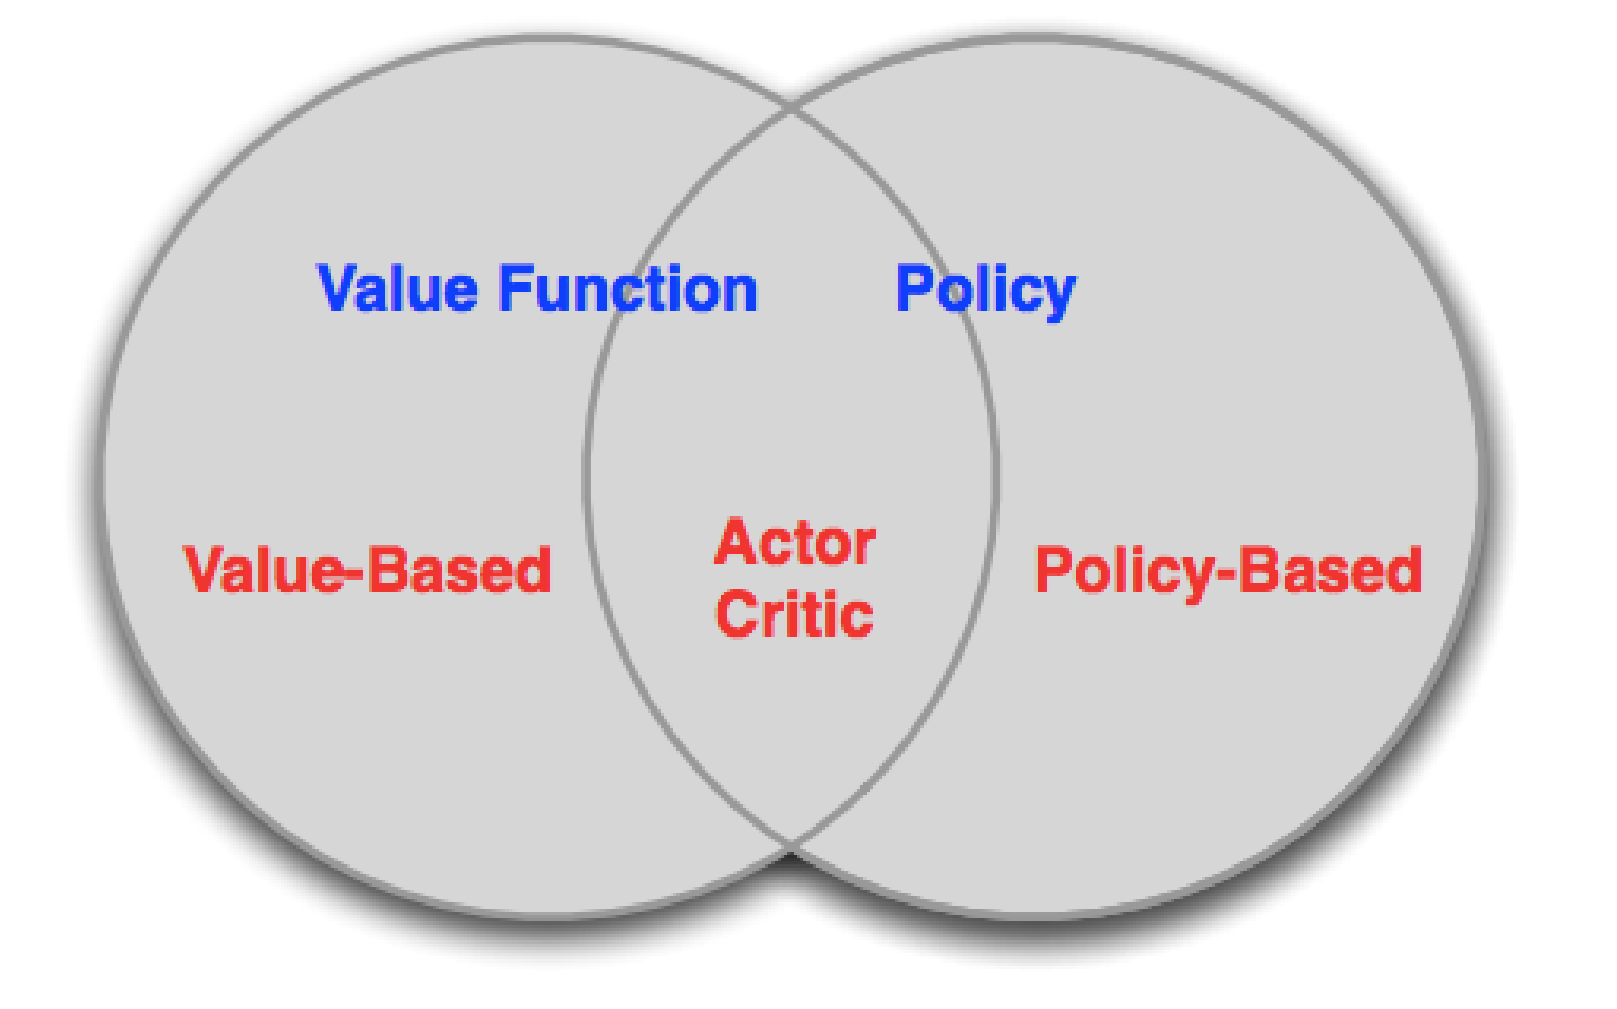
\includegraphics[width=1.0\textwidth,height=1.0\textheight,keepaspectratio]{images/policygrad+reinforce+actor/a2c_2.png}
    \end{figure}
\end{column}
\end{columns}
\end{frame}


\section{Policy Gradient vs. Q-Learning}
\begin{frame}{Policy Gradient vs. Q-Learning}
\begin{itemize}
    \item Policy gradient and Q-learning use two fundamentally different representations: policies and value functions.
    \item Advantage of both methods: no need to model the environment.
    \pause
    \item \textbf{Policy Gradient: Pros and Cons}
    \begin{itemize}
        \setlength{\itemsep}{-0.25em}
        \item \textbf{Pros:} Unbiased estimate of the gradient of expected return.
        \item Can handle large action spaces (since only one action needs to be sampled).
        \item \textbf{Cons:} High variance updates (leads to poor sample efficiency).
        \item Does not perform credit assignment effectively.
    \end{itemize}
    \pause
    \item \textbf{Q-Learning: Pros and Cons}
    \begin{itemize}
        \setlength{\itemsep}{-0.25em}
        \item \textbf{Pros:} Lower variance updates, more sample efficient.
        \item Performs credit assignment.
        \item \textbf{Cons:} Biased updates due to function approximation.
        \item Difficult to handle large action spaces (since the maximum over actions must be computed).
    \end{itemize}
\end{itemize}
\end{frame}
